\subsection{Infinite plate with a circular hole}
\paragraph{}
In this example, an infinite plate with a traction free hole under uniaxial tension $(\sigma = 1 N/m^2 )$ along x-axis (see fig.~\ref{qdt_fig:ex_chole_geo_bc}) is considered.
$L$ is taken as $20$ and $r$ is $5$.
The material properties are: Young’s modulus $E = 100 N/m^2$ and Poisson’s ratio $\nu = 0.3$.
    \begin{figure}[H]
        \centering
        \scalebox{0.5}{
            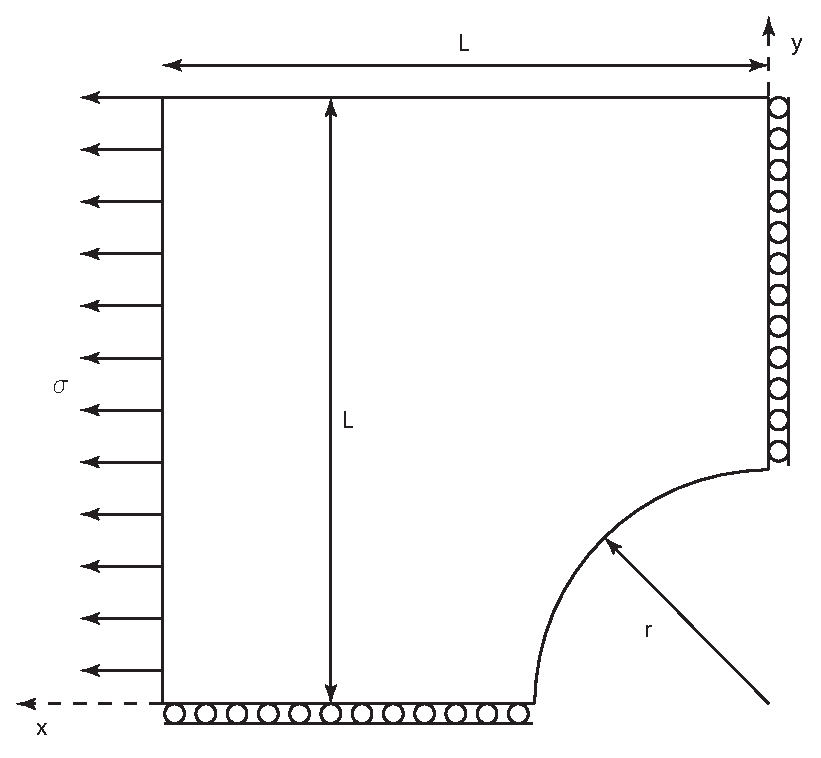
\includegraphics{quadtree/ex_images/qdt_chole_quat_geo_bc.eps}
        }
        \caption{ Infinite plate with a circular hole: geometry and boundary conditions}
        \label{qdt_fig:ex_chole_geo_bc}
    \end{figure}
    
The exact solution of the principal stresses in Cartesian coordinate $(r,\theta)$ is given by \cite{Sukumar2001} in eq.~\ref{iso_eq:ex_chole_stress_sol}.
The closed form displacement in Cartesian coordinate is given in eq.~\ref{iso_eq:ex_chole_disp_sol}.
\paragraph{}
Geometry of the example will be extracted from the iges file drawn in AutoCAD (fig.~\ref{qdt_fig:ex_chole_cad}).
    \begin{figure}[H]
        \centering
        \scalebox{0.4}{
            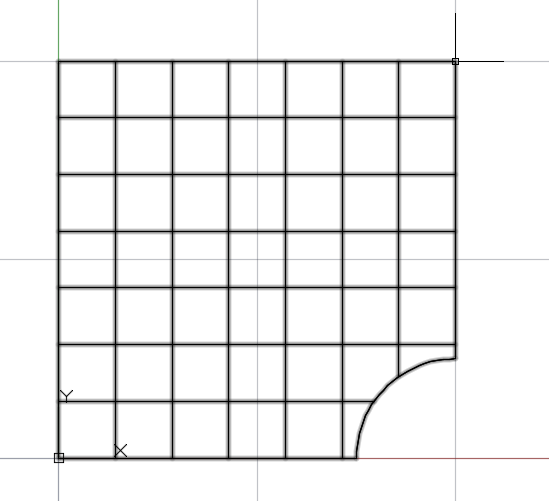
\includegraphics{quadtree/ex_images/ex_chole_cad.png}
        }
        \caption{Infinite plate with a circular hole: CAD drawing}
        \label{qdt_fig:ex_chole_cad}        
    \end{figure}


Generated background mesh, coloring and the final result with $res=32$, $s_{max}=4$ and $s_{min}=1$ are shown in fig.~\ref{qdt_fig:ex_chole_background_mesh}, fig.~\ref{qdt_fig:ex_chole_mesh_coloring} and fig.~\ref{qdt_fig:ex_chole_mesh_final}.

\begin{figure}
    \centering
    \scalebox{0.4}{
        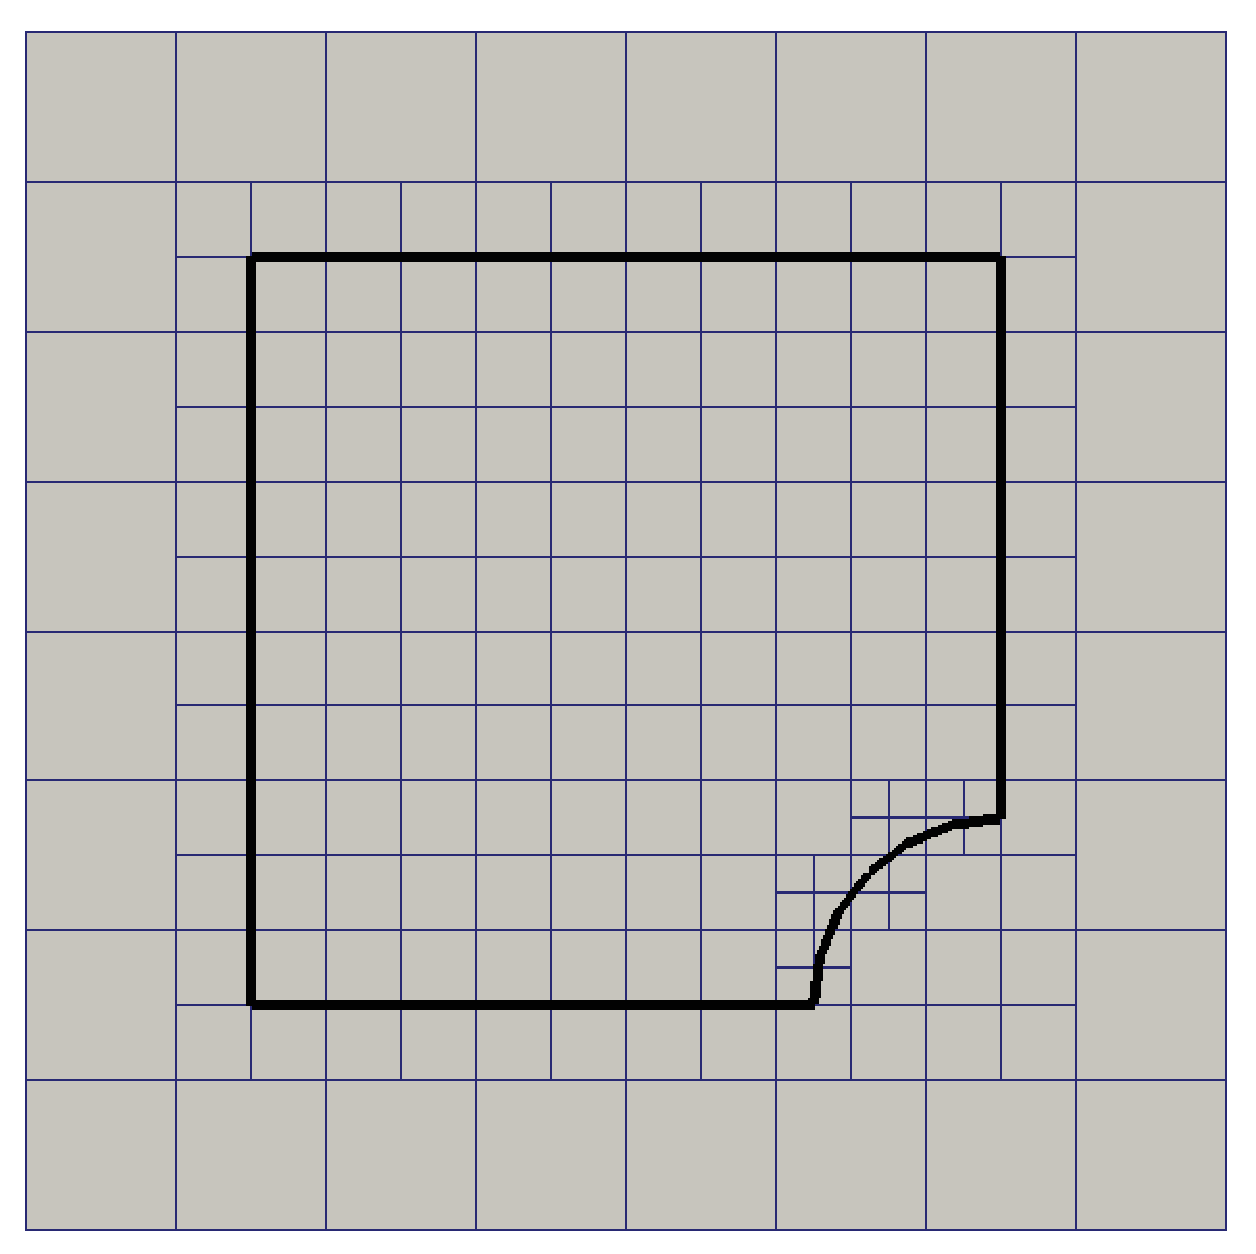
\includegraphics{quadtree/ex_images/ex_chole_background.eps}
    }
    \caption[Background mesh of infinite plate with a circular hole]{Background mesh of infinite plate with a circular hole : Bold lines represents the input geometry}
    \label{qdt_fig:ex_chole_background_mesh}
\end{figure}

\begin{figure}
    \centering
    \scalebox{0.4}{
        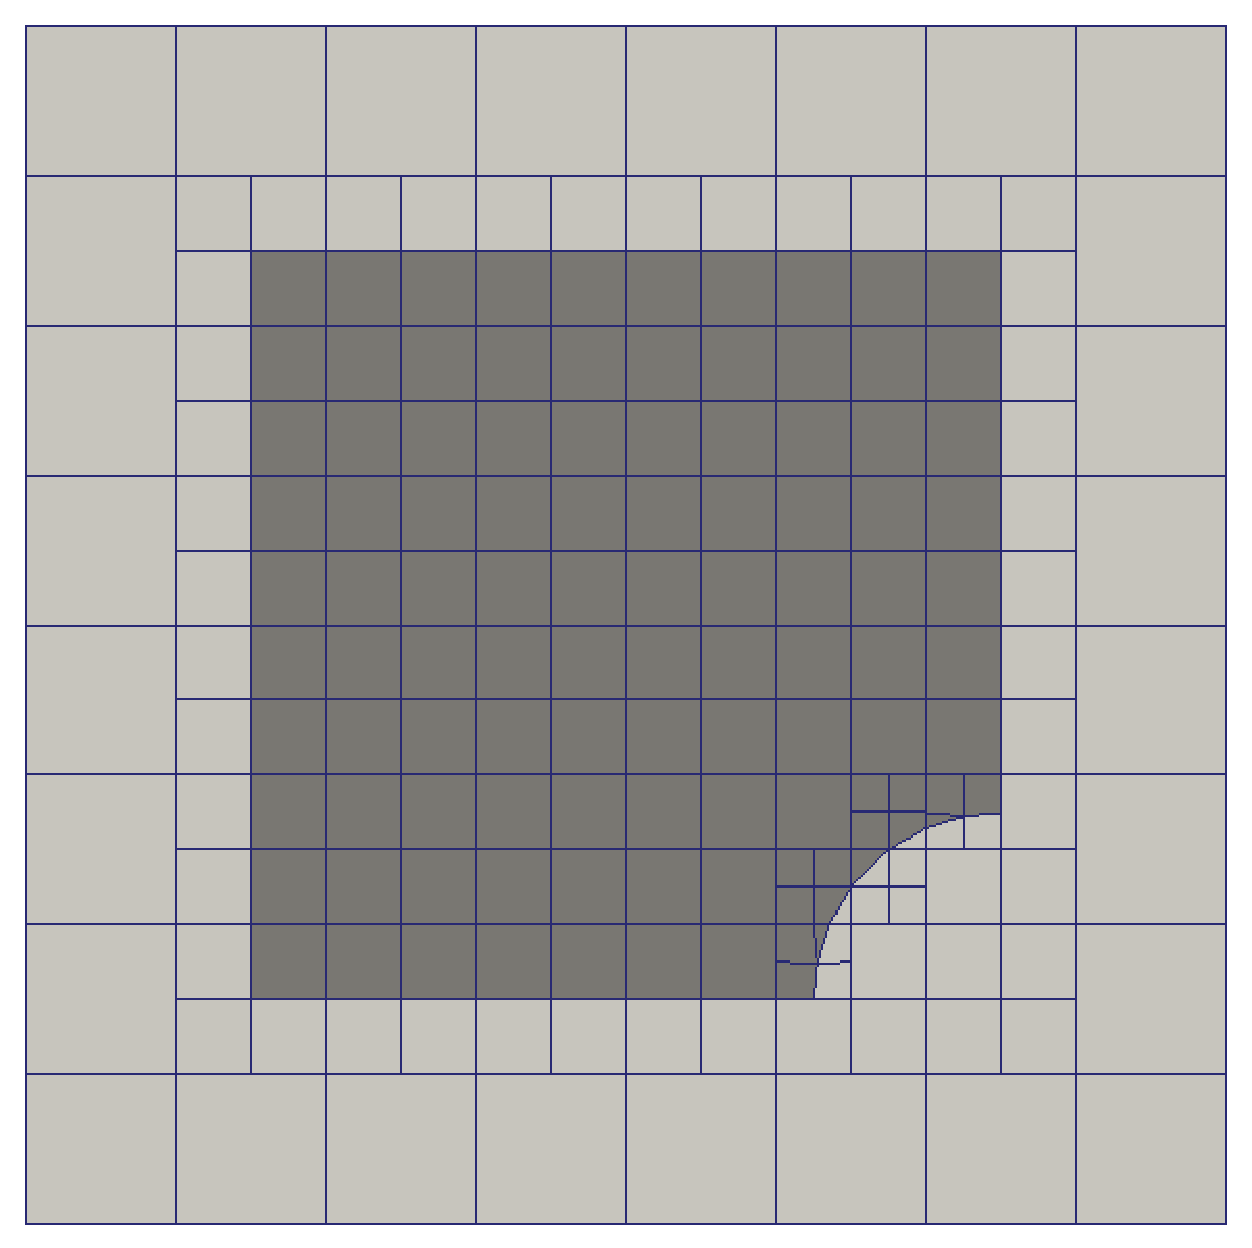
\includegraphics{quadtree/ex_images/ex_chole_coloring.eps}
    }
    \caption[Mesh coloring of infinite plate with a circular hole]{Mesh coloring of infinite plate with a circular hole : Grey area represents the plate}
    \label{qdt_fig:ex_chole_mesh_coloring}
\end{figure}

\begin{figure}
    \centering
    \scalebox{0.4}{
        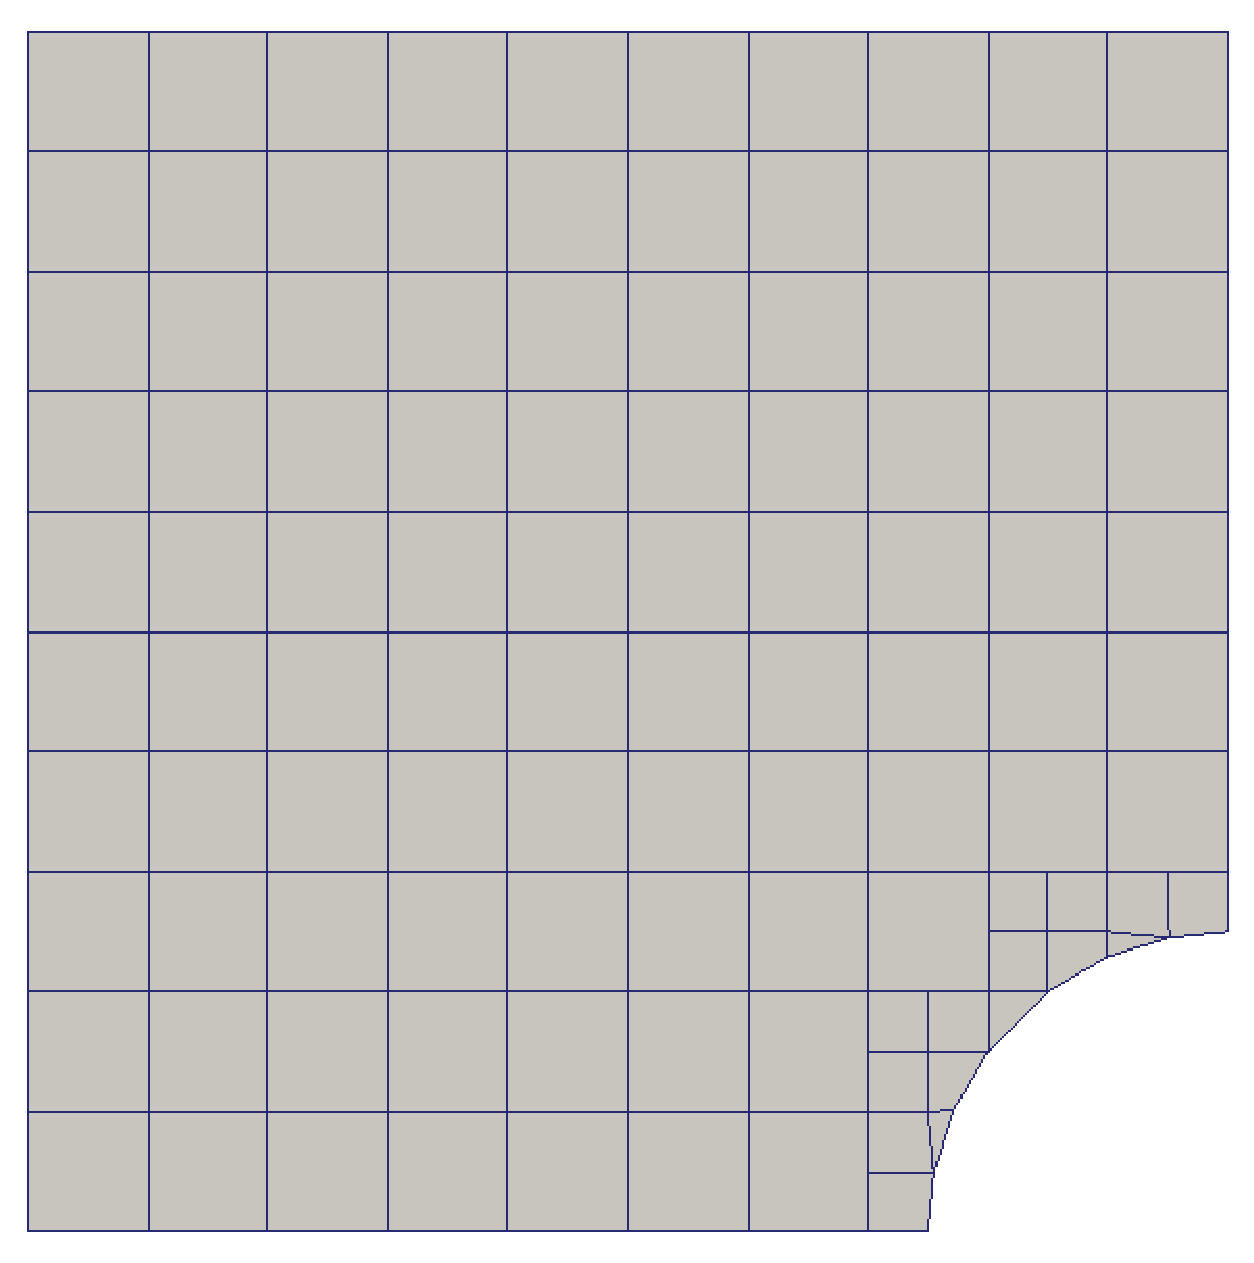
\includegraphics{quadtree/ex_images/ex_chole_mesh_262.eps}
    }
    \caption[Final mesh of infinite plate with a circular hole]{Final mesh of infinite plate with a circular hole}
    \label{qdt_fig:ex_chole_mesh_final}
\end{figure}
% 262 - 0.0112 (32-4/5-4)
% 290 - 0.0101 (64-4/5-4)
% 876 - 0.0036216 (128-4/8-4)
% 3280- 0.0010068 (256-4/15-4)
\paragraph{}
Mesh with different parameters are plotted in fig.~\ref{qdt_fig:ex_chole_mesh_all} and the convergence study is plotted in fig.~\ref{qdt_fig:ex_chole_mesh_conv}

\begin{figure}[H]
    \begin{subfigure}[b]{1\linewidth}
        \centering
        \scalebox{0.4}{
            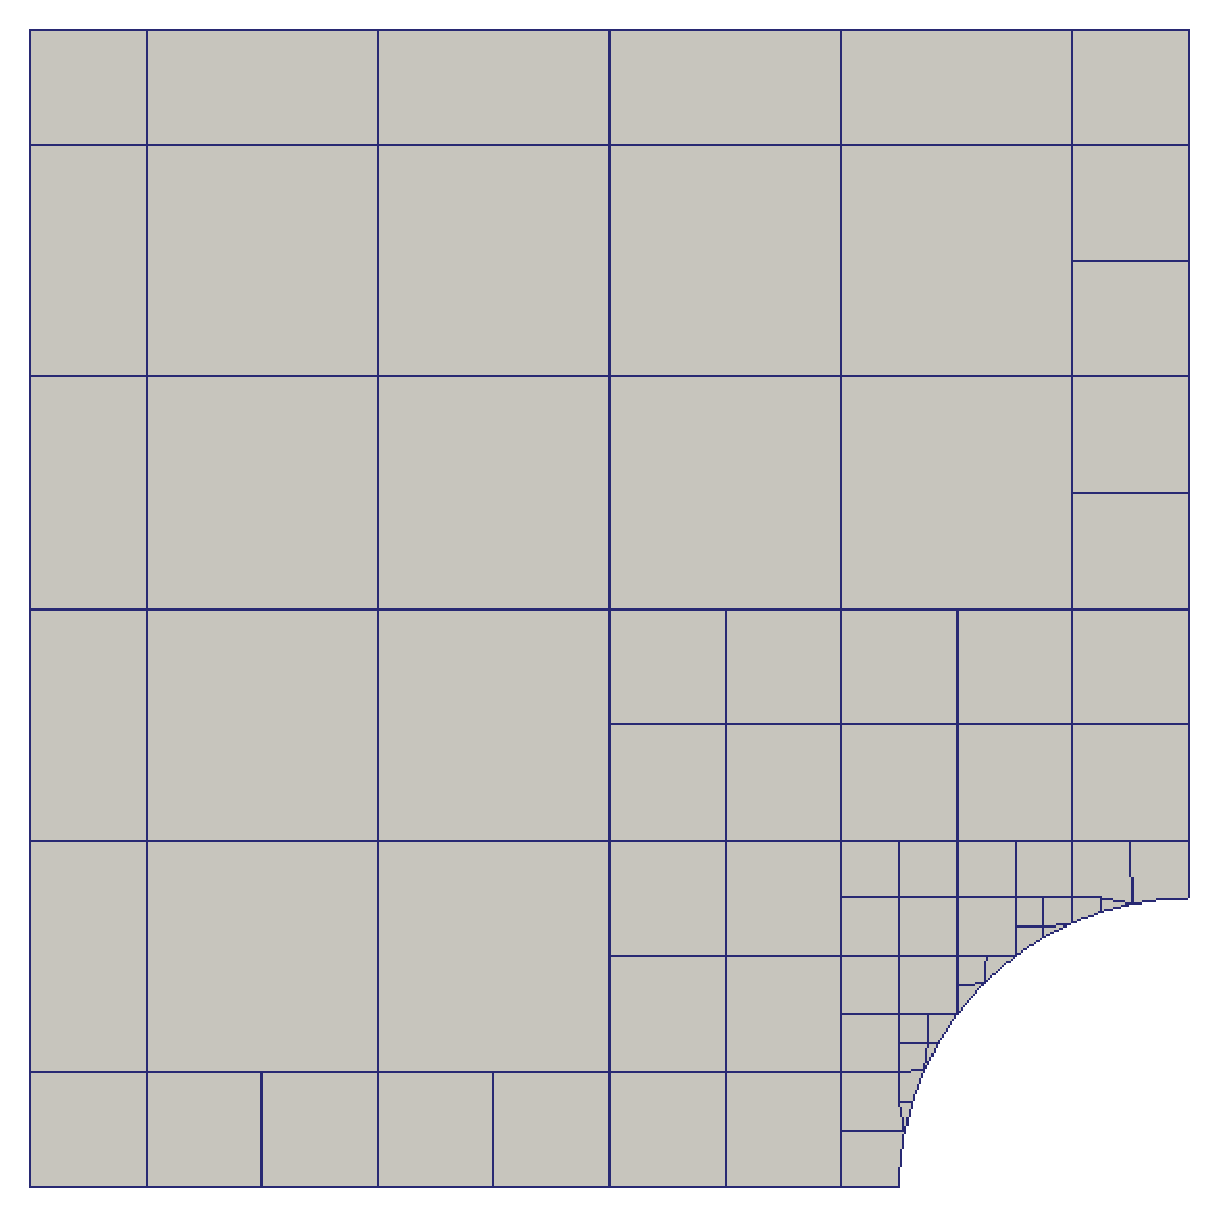
\includegraphics{quadtree/ex_images/qdt_chole_64_8.eps}
        }
        \caption{Mesh with $res=64$, $s_{max}=8$, 152 DOFs}
    \end{subfigure}
    \\
    \begin{subfigure}[b]{1\linewidth}
        \centering
        \scalebox{0.4}{
            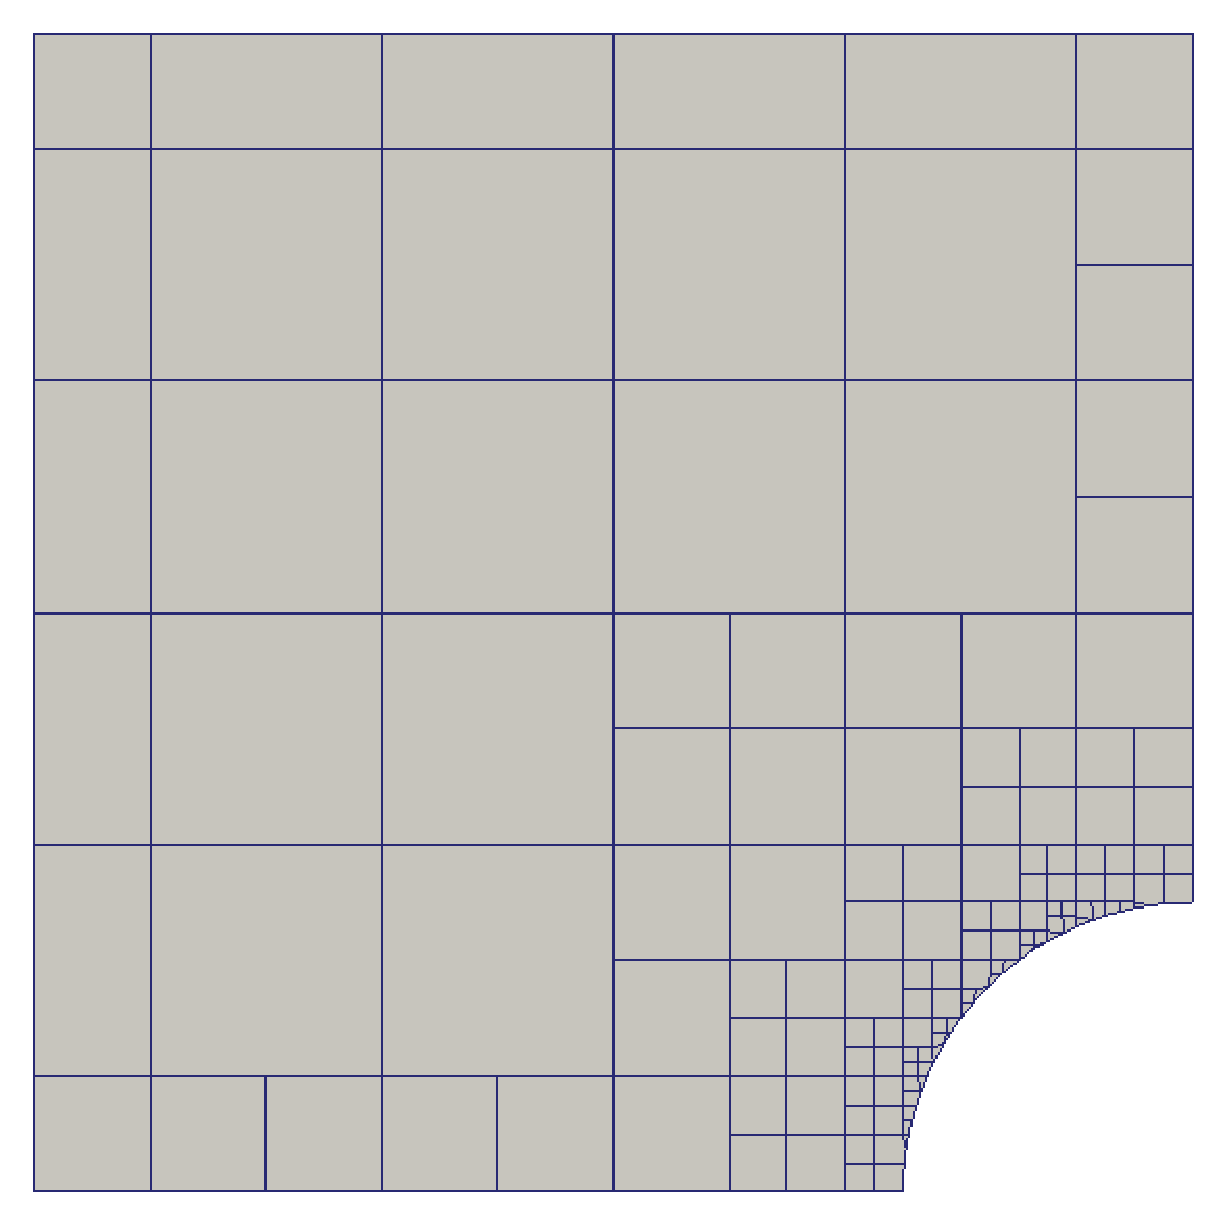
\includegraphics{quadtree/ex_images/qdt_chole_128_16.eps}
        }
        \caption{Mesh with $res=128$, $s_{max}=4$, 272 DOFs}
    \end{subfigure}
\end{figure}

\begin{figure}[H]\ContinuedFloat
    \begin{subfigure}[b]{1\linewidth}
        \centering
        \scalebox{0.5}{
            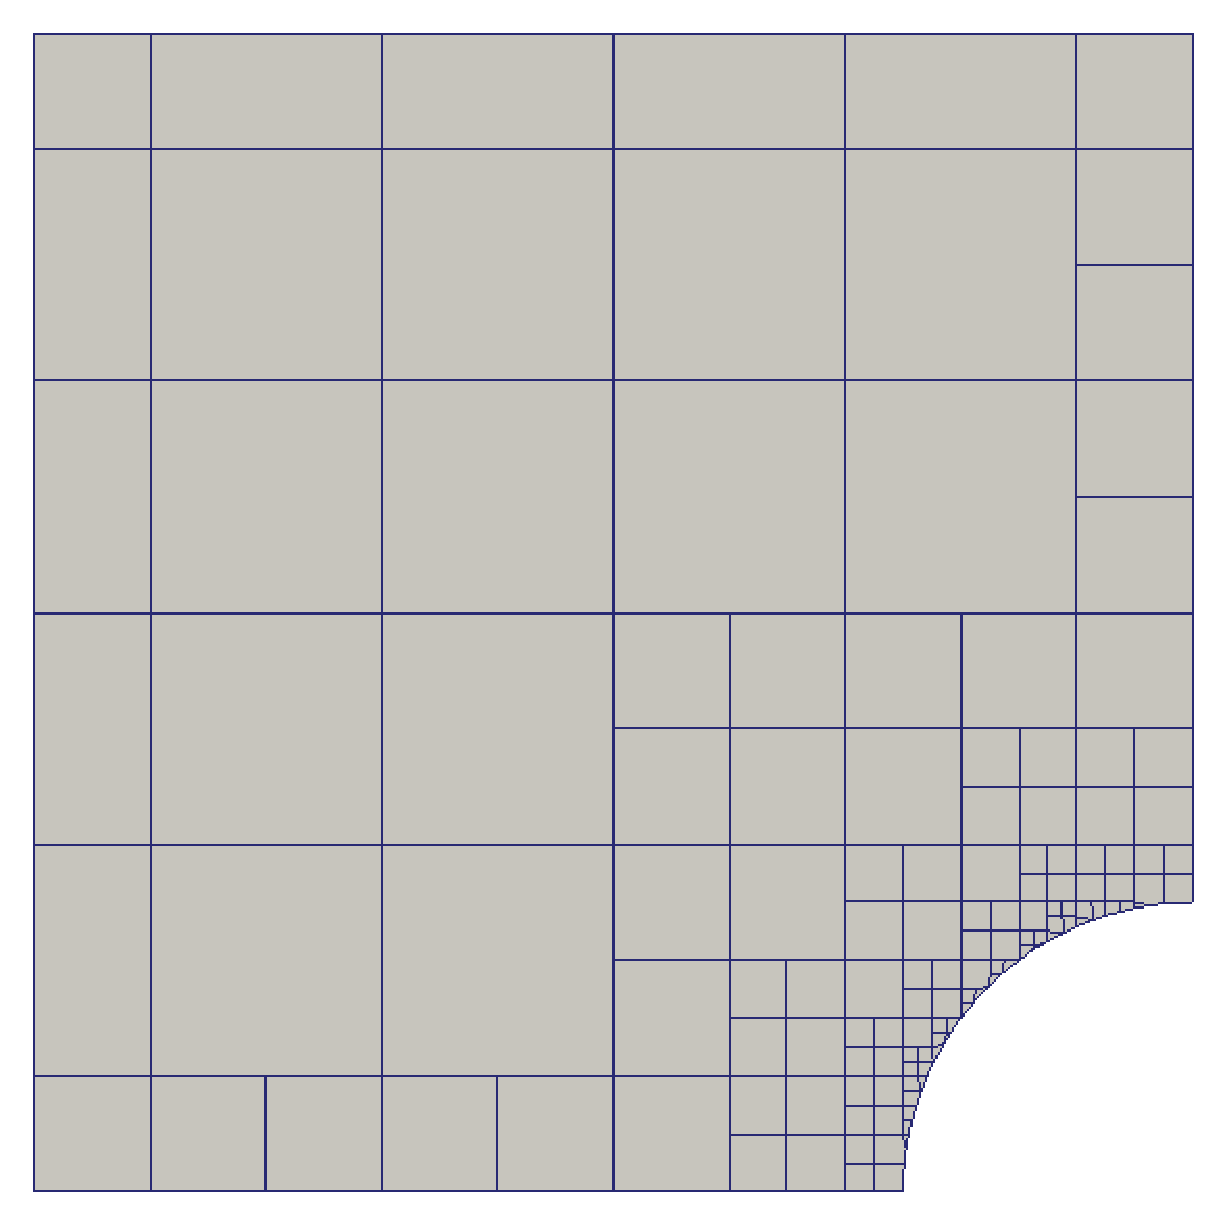
\includegraphics{quadtree/ex_images/qdt_chole_128_16.eps}
        }
        \caption{Mesh with $res=128$, $s_{max}=16$, 488 DOFs}
    \end{subfigure}
    \caption[Mesh of the infinite plate with a circular hole]{Mesh of infinite plate with a circular hole}
    \label{qdt_fig:ex_chole_mesh_all}
\end{figure}


\begin{figure}[H]
    \centering
    \scalebox{0.6}{
        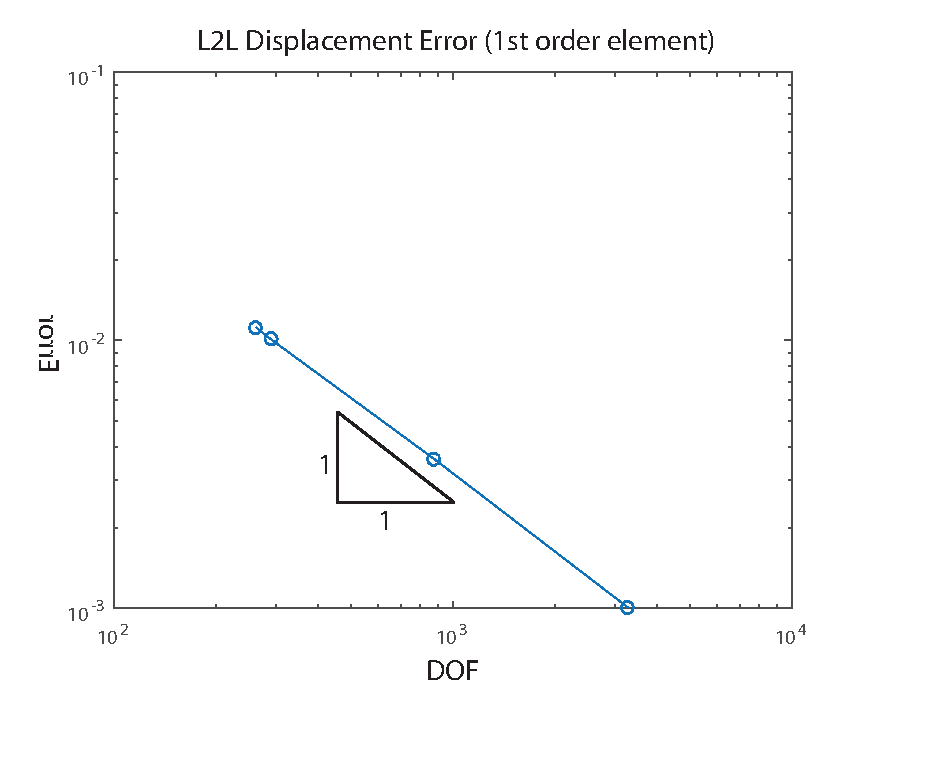
\includegraphics{quadtree/ex_images/ex_chole_conv.eps}
    }   
    \caption[Convergence of the infinite plate with a circular hole]{Convergence of the infinite plate with a circular hole}
    \label{qdt_fig:ex_chole_mesh_conv}
\end{figure}

\pagebreak